\newSec[ImplPlugCall]{\textit{calling} \Pack}{3}

Dieses \Pack\ wurde eingeführt, um die Erzeugung neuer \ROS-\Msg[s] zu umgehen. Ferner bildet die Struktur dieser Klassen einen \textit{pull Observer} ab.
Die aufgerufene Methode erhält den Pointer auf die aufrufende Klasse und kann hiermit eine Entscheidung über weitere Aktionen treffen.

\note{Dieses \Pack\ entspricht nicht den Grundsätzen einer \ROS-Programmierung und ist daher nicht weiter zu nutzen. Die Beschreibung dient an dieser Stelle dem Verständnis des Einsatzes dieser Klassen im \textit{coex} \Pack\ und wird darüber hinaus nicht weiter eingesetzt.}



\begin{figure}[ht!]
\vspace{0.25cm}
\begin{center}
\fbox{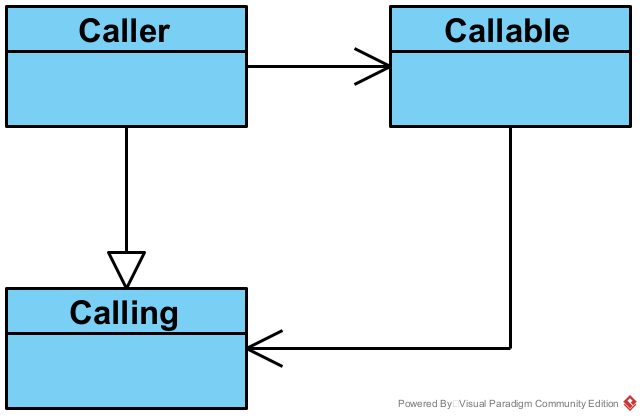
\includegraphics[width=6cm]{Pictures/calling_Pkg.png}}
\caption{Klassendiagramm des \textit{calling} \Pack[s]}
\label{fig:PackCaller}
\end{center}

\vspace{0.25cm}
\end{figure}


